\documentclass[12pt]{article}
\usepackage{fullpage,amsmath,amsfonts,mathpazo,microtype,nicefrac,graphicx,fancyhdr,listings,hyperref,csvsimple}
\graphicspath{ {figures/} }
\author{Akhil Ketkar \hspace{4.1cm} Arjun Sanghvi \\
	\texttt{akhilketkar@g.harvard.edu} \hspace{1cm} \texttt{asanghvi@g.harvard.edu}}
\pagestyle{fancy}
\fancyhf{}
\rhead{AM205 2014 Final Project -- AK AS}
\lstset{
	language=Python,
	showstringspaces=false,
	formfeed=\newpage,
	tabsize=4,
	commentstyle=\itshape,
	basicstyle=\ttfamily\scriptsize,
	morekeywords={models, lambda, forms}
}
\headsep = 25pt
        
% Macro definitions
\newcommand{\N}{\mathbb{N}}
\newcommand{\Z}{\mathbb{Z}}
\newcommand{\Q}{\mathbb{Q}}
\newcommand{\R}{\mathbb{R}}
\newcommand{\p}{\partial}
\newcommand{\Trans}{\mathsf{T}}

% include graphics
% \includegraphics[width=0.8\textwidth]{figureProb40}

% include code 
% 

% include csv
% \csvautotabular{charge_output.csv}


\title{Network Analysis of Enron Email Data}
\begin{document}

\begin{figure}
\centering

\includegraphics[width=15cm]{EnronNetwork}
\end{figure}

\maketitle


\clearpage

\section{Introduction}
	The world has never been more connected. The Internet is nearly ubiquitous and acts as both a catalyst for human interaction and a lens through to which study it. Increased generation and accessibility of data, in addition to the proliferation of massive social networks, has led to substantial network analysis research in the past two decades.
	
	Graph theory offers a natural translation of network structure to mathematical formulation. The fundamental characteristics of graphs are the existence of nodes and the connections between them (edges). For example, one network that we interact with on a daily basis is defined by our communication through e-mail. In the graph theoretic translation, we can represent e-mail senders and receivers (people, organizations, etc.) as nodes and e-mail exchanges between two parties as edges linking them together.
	
	In this paper, we examine structural properties of the Enron email network to better understand the organization and dynamics of the corporation in its final tumultuous years. The Enron e-mail corpus was initially released by the Federal Energy Regulatory Commission (FERC) in 2003 as part of its legal investigation into the company \cite{ferc}. The information released consisted of the sender, receiver, date, and text of over 600,000 messages from 158 employees. In taking the unprecedented step of releasing what was presumed to be confidential information, the FERC has allowed for an intimate look into the business practices and social hierarchy of a company notorious for its aggressive corporate culture.
	
Previous analyses of the Enron dataset include investigation of graph theoretic and spectral characteristics, classification and sorting of e-mail by sender-receiver relationship and chronology, database construction, and Natural Language Processing \cite{Diesner, Chapanond, Priebe}. Here, we explore several metrics of centrality to elucidate key figures in the network and evaluate the method results in the context of the corporate hierarchy. Furthermore, we employ spectral partitioning, modularity maximization, and singular value decomposition for clustering and community detection. Finally, we consider the time evolution of major network characteristics, such as average path length and diameter, on the scale of months. This level of granularity over the three-year period captures significant shifts in network dynamics that can be corroborated with the true timeline of events. 

\section{Brief Background on Enron}
Enron was formed in 1985 when energy utility InterNorth Inc. acquired Houston Natural Gas. Throughout the 1990s, the company was lauded for its innovative business practices. In addition to building and operating infrastructure to support power distribution, the company engaged in aggressive trading practices in energy futures and created new financial products entirely. It would later be revealed that the company played a direct role in the California electricity crisis of 2000, which resulted in rolling blackouts across the state. Recordings of phone conversations between Enron employees and utility operators indicate that Enron took power plants offline during peak energy usage to induce artificial shortages, which spiked energy prices and allowed for lucrative trading opportunities. Nevertheless, by additionally leveraging a burgeoning Internet during the dot-com era, the company eventually became one of the largest in the United States, and achieved a market value of nearly 70 billion dollars.

Of course, market valuation need not reflect intrinsic value. In 2001, the company became mired in an investigation of its accounting practices. The investigation revealed hundreds of millions of dollars in debt that had been attributed to subsidiary companies that Enron had created precisely for that purpose. A conviction of fraud followed, and then bankruptcy. The revelations that unfolded over the next several years revealed an expansive network of oblivious and complicit individuals, including high ranking policy makers and one of the largest accounting firms of the time, Arthur Andersen LLP. Several top executives, including CEOs Kenneth Lay and Jeff Skilling, were indicted on criminal charges, and a few are currently serving prison terms. The company has become an iconic representation of corporate corruption and greed in American culture \cite{npr}.

\section{Data and Resulting Graphs}
	\subsection{Dataset}
	There are several versions of the Enron email dataset. The version that we are utilizing for this paper comes from the work of Jitesh Shetty and Jafar Adibi \cite{shetty} at ISI. Shetty and Adibi cleaned the dataset by dropping emails that were blank, duplicates of unique emails, had junk data, or were returned by the system due to transaction failures. The final dataset consists of 252,759 emails in 3000 user defined folders from 151 people. Shetty and Abidi loaded the information into a MySql database that contains four tables containing information about the employees, messages, recipients and reference information. 
	
	We chose this version of the dataset mainly because it is has been structured into a relational database. Unfortunately Shetty and Adibi's website (which was used as a source by a number of papers) was taken down recently. So we retrieved a copy of the the data from Joel Pfeiffer's website \cite{pfeiffer}. In addition to the email data, we also used data on the positions and specific roles of various employees from Youngser Park\cite{park}.
	
	We made several modifications to the dataset to arrive at the version that was used in the analysis such as: normalizing the email addresses for all the employees, adding missing emails addresses, removing emails that were not sent from other employees etc. We then incorporated the employee position data into the email data to create the final version of the dataset. 

	\subsection{Graphs}
	All subsequent analysis in the paper relies on the network representation of the dataset mentioned above. The nodes of the network are the employees of Enron and the edges represent individual email exchanges. Certain parts of the paper use directed graphs where an edge goes from a sender to the receiver of the email while other parts use undirected graphs where an edge simply denotes an email sent between the two nodes.
	
	This is an example of the network drawn from emails sent in October 2000. In this period Enron's share price was close to its all time highs. \\
	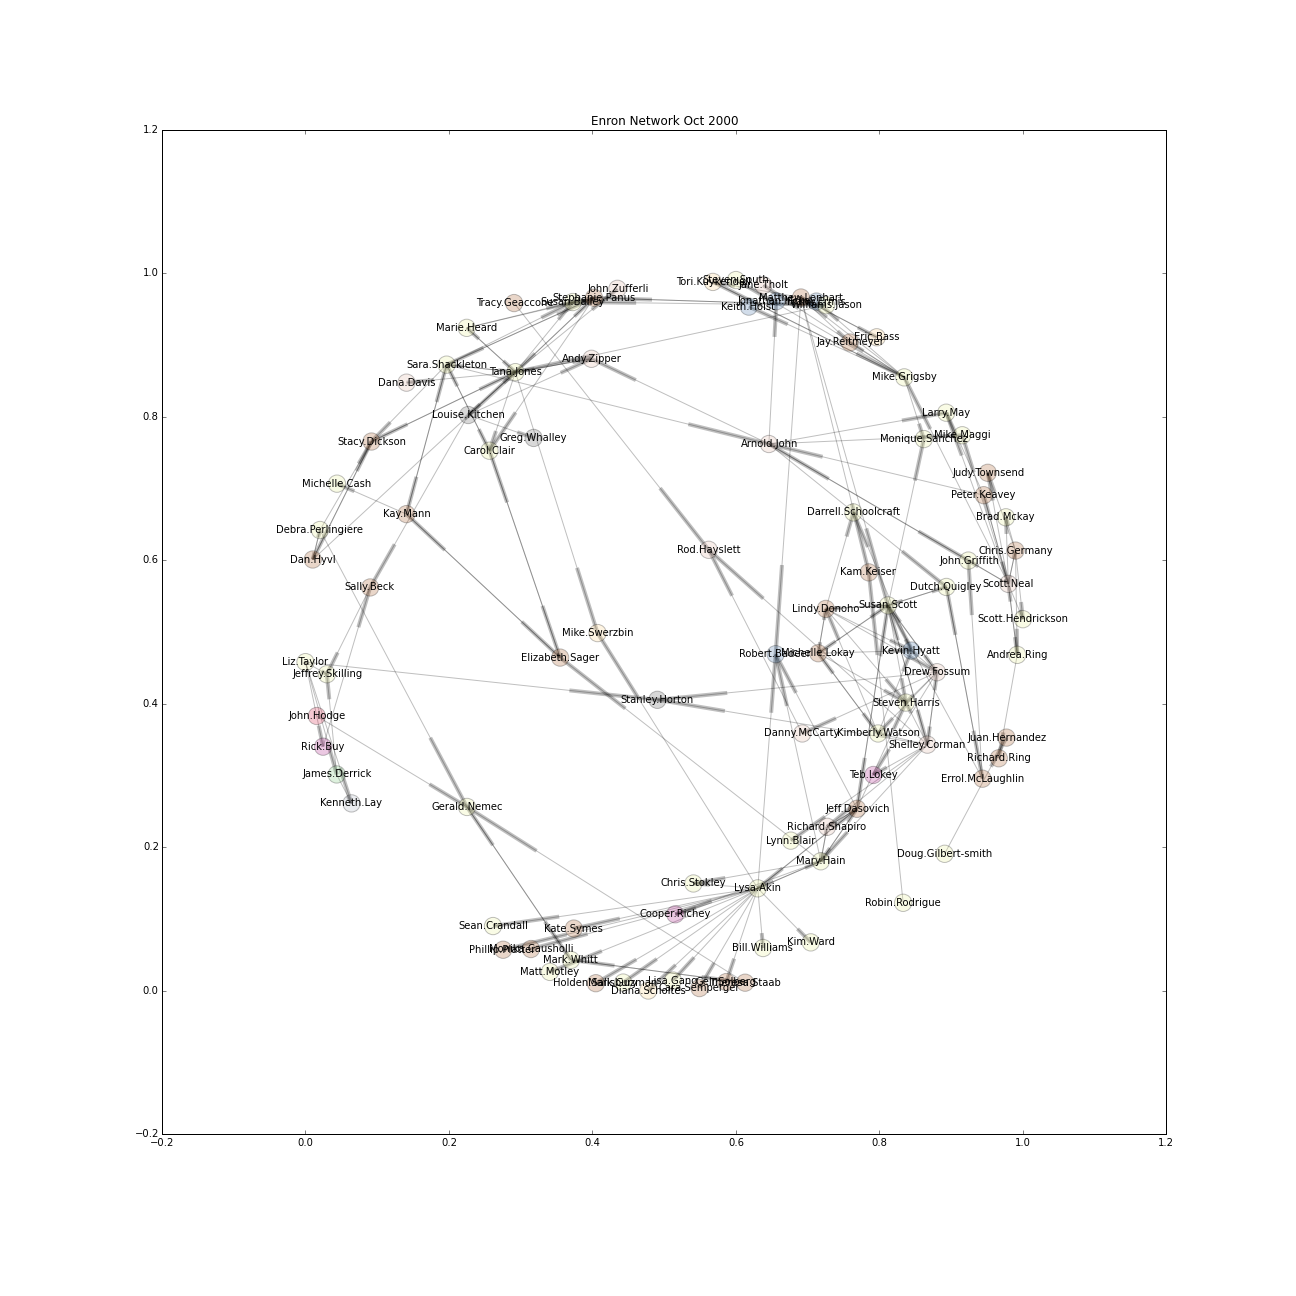
\includegraphics[width=1\textwidth]{figureEnronOct2000}
	
	Compare the network in Oct 2000 to this network created from emails sent in October 2001 at which point the fraud at Enron has been exposed and Enron is nearing bankruptcy.
	
	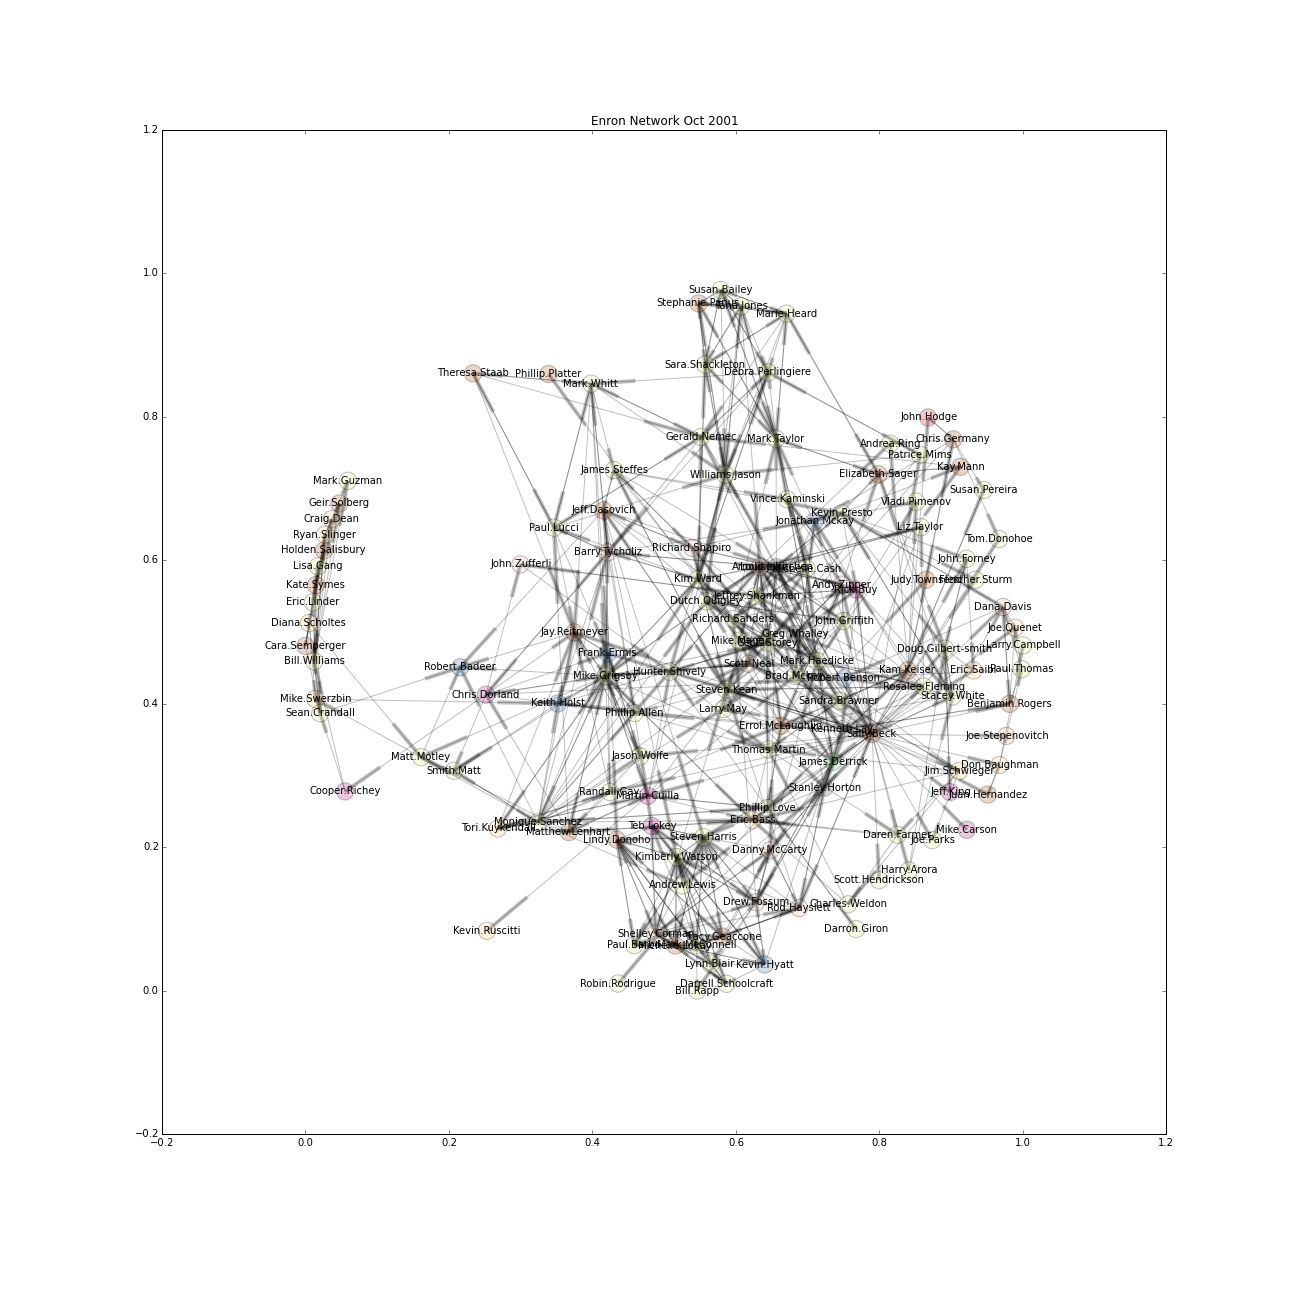
\includegraphics[width=1\textwidth]{figureEnronOct2001}
	
	\subsection{Terminology}
	\begin{enumerate}
		\item $A$ is the adjacency matrix of the network which is $n$ x $n$ for a network with $n$ nodes.
		\item $D$ is the diagonal matrix containing node degrees on it's diagonals
		\item $L$ is the laplacian of the matrix defined as $D - A$
		\item $B$ is the modularity matrix defined as $B_{ij} = A_{ij} - \frac{k_i k_j}{2m}$ where $k_a$ is degree of node $a$
	\end{enumerate}

\section{Centrality Measures} One of the key questions one can ask about an information network such as the Enron email network is: Who are the most important actors in the network? There are various measures of centrality one can use to answer that question.	
	\subsection{Eigenvector Centrality} Eigenvector based centrality measures are based on the idea that a node is important if it is connected to other important nodes. Let $A$ be the adjacency matrix of a graph and $x$ the vector of centrality measures. We would like the centrality of each node to be proportional to the centralities of all the nodes connected to it. In matrix form then we would like vector $x$ to satisfy the equation
		\begin{equation}
			A x = \kappa x
		\end{equation}
		Thus $x$ is an eigenvector of the matrix $A$. Even though all eigenvectors of $A$ satisfy the above equation, the eigenvector corresponding to the largest eigenvalue is used in practice. In order to compute the largest eigenvalue we use the power method.
		
        \begin{table}[h]
        \caption{Employees with Greatest Eigenvector Centrality}
        \centering
        \begin{tabular}{|l|l|l|}
        \hline
        \textbf{Name }          & \textbf{Eigenvector Centrality} & \textbf{Position}                              \\ \hline
        Sally Beck     & 0.238627               & Chief Operating Officer               \\ \hline
        Liz Taylor     & 0.229042               & Administrative Assistant to President \\ \hline
        Louise Kitchen & 0.220102               & President of Enron Online             \\ \hline
        Kenneth Lay    & 0.205464               & CEO                                   \\ \hline
        John Lavorato  & 0.201416               & CEO, Enron America                    \\ \hline
        Mike Grigsby   & 0.156134               & Vice President                        \\ \hline
        Kevin Presto   & 0.148424               & Vice President                        \\ \hline
        Scott Neal     & 0.147877               & Vice President, trader                \\ \hline
        Barry Tycholiz & 0.145584               & Vice President                        \\ \hline
        Arnold John    & 0.145032               & Vice President                        \\ \hline
        \end{tabular}
        \end{table}
	
	Katz centrality and PageRank are small modifications on the idea of eigenvector centrality. This measure identifies several key members of upper management at Enron despite the fact that they don't send or receive a lot of email.
	
	\subsection{Other measures of Centrality}
	
	\subsubsection{Closeness Centrality} For a node $v$, this is defined as the reciprocal of the sum of shortest path distances from $v$ to all other $n-1$ nodes. Perhaps the most intuitive of the centrality measures, the closer a node is to others (in terms of intermediary nodes, or so called degrees of separation), the greater its closeness centrality.
	
	\begin{equation}
			C(v) = \frac{n-1}{\sum\limits_{v=1}^{n-1} d(u,v)}
	\end{equation}
	where $n$ is the number of nodes in the network and $d(u,v)$ is the shortest path length between node $u$ and $v$.

        \begin{table}[h]
        \caption{Employees with Greatest Closeness Centrality}
        \centering
        \begin{tabular}{|l|l|l|}
        \hline
        \textbf{Name} & \textbf{Closeness Centrality} & \textbf{Position}                     \\ \hline
        Liz Taylor        & 0.653509                      & Administrative Assistant to President \\ \hline
        Sally Beck        & 0.626050                      & Chief Operating Officer               \\ \hline
        John Lavorato     & 0.618257                      & CEO, Enron America                    \\ \hline
        Louise Kitchen    & 0.598394                      & President of Enron Online             \\ \hline
        Kenneth Lay       & 0.579767                      & CEO                                   \\ \hline
        Jeff Dasovich     & 0.541818                      & Executive, Government Relations       \\ \hline
        Kevin Presto      & 0.528369                      & Vice President                        \\ \hline
        Susan Scott       & 0.526502                      & Assistant Trader                      \\ \hline
        Mike Grigsby      & 0.520979                      & Vice President                        \\ \hline
        Arnold John       & 0.520979                      & Vice President                        \\ \hline
        \end{tabular}
        \end{table}
        
        Again, several important figures in the business structure are highlighted.  
        
	\subsubsection{Betweenness Centrality} Betweenness centrality of a node is the sum of the fraction of all-pairs shortest paths that pass through that node. It could be thought of as a measure of the role that a node plays in the transfer of information.
	
	\begin{equation}
			B(v) = \sum\limits_{s\neq v \neq t} \frac{\sigma_{st}(v)}{\sigma_{st}}
	\end{equation}

where $\sigma_{st}$ is the number of shortest paths from $s$ to $t$ and $\sigma_{st}(v)$ is the number of those paths that go through $v$.
	        
        \begin{table}[h]
        \caption{Employees with Greatest Betweenness Centrality}
        \centering
        \begin{tabular}{|l|l|l|}
        \hline
        \textbf{Name}  & \textbf{Betweenness Centrality} & \textbf{Position}                       \\ \hline
        Louise Kitchen & 0.100766                        & President of Enron Online               \\ \hline
        Susan Scott    & 0.069708                        & Assistant Trader                        \\ \hline
        Mike Grigsby   & 0.060098                        & Vice President                                        \\ \hline
        Kenneth Lay    & 0.048120                        & CEO                                     \\ \hline
        Kim Ward       & 0.046483                        & Associate Director, Enron North America \\ \hline
        Jeff Dasovich  & 0.045877                        & Executive, Government Relations         \\ \hline
        Liz Taylor     & 0.043397                        & Administrative Assistant to President   \\ \hline
        Sally Beck     & 0.043037                        & Chief Operating Officer                 \\ \hline
        Kevin Presto   & 0.040577                        & Vice President                          \\ \hline
        Bill Williams  & 0.037401                        & Trader                                  \\ \hline
        \end{tabular}
        \end{table}
        
        The three centrality measures presented here have significant overlap in results despite different underlying methodologies. This may be evidence of a particularly entrenched hierarchical structure. Perhaps most interestingly, the most significant figure in the network, CEO Kenneth Lay, is deemed central by all three measures even though he exchanged very few e-mails relative to the rest of the network.
        
\newpage
\section{Communities} The basic goal of community detection is to separate the network into groups of vertices that have few connections between them. The following discussion is based on Mark Newman's work \cite{newman}. 

	
	Cut size is a simple metric that can be used to find communities in a network. The cut size is simply the number of edges you have to remove from the network so that the two groups of nodes become disconnected. 
	\begin{equation}
		R = \frac{1}{2} \sum_{i,j in different groups} A_{ij}
	\end{equation}
	where the factor of $\frac{1}{2}$ compensates for the fact that each edge appears twice in the adjacency matrix.

	Modularity is another (arguably better) measure. The idea is that we find  the fraction of edges that run between vertices of the same type, and then we subtract from that figure the fraction of such edges we would expect to find if edges were positioned at random without regard for vertex type \cite{newman}. When the fraction of edges between vertices of the same type is significantly greater than what would be expected at random, we can say that the network exhibits high homophily. The number of edges that run between nodes of the same type is given by
	\begin{equation}
		\sum_{edges (i,j)} \delta (c_i, c_j) = \frac{1}{2} A_{ij} \delta (c_i, c_j)
	\end{equation}
	where $c_i$ and $c_j$ are the classes of nodes and $\delta (m,n)$ is the Kronecker delta which is equal to 1 if $m = n$ and 0 otherwise.
	
	
	The expected number of edges between nodes of the same type is given by
	\begin{equation}
		\frac{1}{2} \sum_{i,j} \frac{k_i k_j}{2m} \delta (c_i,c_j)
	\end{equation}
	where $k_i$ denotes the number of edges of node $i$ (it's degree) and $m$ is the total number of edges in the network. Subtracting (3) from (2) gives us modularity $Q$
	\begin{equation}
		Q = \frac{1}{2m} \sum_{i,j} \left( A_{ij} - \frac{k_i k_j}{2m} \right) \delta (c_i,c_j)
	\end{equation}

	\subsection{Partitioning using Cut Size} 
	We can use these ideas to find communities within a network.  
	
	Let us define quantities $s_i$ for each vertex $i$, which represent the division of the network: 
	\begin{align}
		s_i = +1 \text{ if node belongs in group 1} \\
		s_i = -1 \text{ if node belongs in group 2}
	\end{align}
	Then
	\begin{align}
		\frac{1}{2} (1 - s_i s_j) = 1 \text{ if i and j are in the same group} \\
		\frac{1}{2} (1 - s_i s_j) = 0 \text{ if i and j are in different groups}
	\end{align}
	
	This allows us to rewrite equation 2 for cut size as
	\begin{equation}
		R = \frac{1}{4} \sum_{ij} A_{ij} (1- s_i s_j)
	\end{equation}
	
	Simplifying the above equation and using the fact that $\sum_j A_{ij} = k_i$ we get
	\begin{equation}
		R = \frac{1}{4} \sum_{ij} (k_i \delta_{ij} - A_{ij}) s_i s_j = \frac{1}{4} \sum_{ij} L_{ij} s_i s_j
	\end{equation}
	where $L$ is the Laplacian of the matrix. We can rewrite this equation in matrix form as 
	\begin{equation}
		R = \frac{1}{4} s^T L s
	\end{equation}
	where $s$ is the vector of all $s_i$. Equation 12 gives us a optimization problem: find $s$ such that the quantity $R$ is minimized. $s$ is constrained to only have values that are +1 or -1. \\
	
	This turns out to be a very difficult problem to solve so we relax some of the constraints on $s$. $s$ is allowed to take any value subject to $|s|$ = $\sqrt{n}$ where $n$ is the number of nodes and $1^T s = n_1 - n_2 $ where $n_1$ and $n_2$ are the sizes of the partitions we need. 
	
	We can differentiate with respect to $s$ and introduce two Lagrange multipliers to solve this problem
	\begin{equation}
		\frac{\partial}{\partial s_i} 
			\left[ 
			\sum_{jk} L_{jk} s_j s_k 
			+ \lambda \left( n - \sum_j s_j^2 \right)
			+ 2 \mu \left( (n_1 - n_2) - \sum_i s_j \right)
			\right] = 0 
	\end{equation}
	
	This results in
	\begin{equation}
		L s = \lambda s + \mu 1 
	\end{equation} \\
	
	It is easy to see that the vector 1 is an eigenvector of a Laplacian matrix since the sum of the off-diagonal entries of a Laplacian is the degree which is 0 minus the diagonal element of the matrix. Knowing this allows us to compute $\mu = - \frac{n_1 - n_2}{n} \lambda$. \\
	
	If we define a new vector $x$ = $s + \frac{\mu}{\lambda} 1$ we can see that $L x = \lambda x$. We now need to pick a $\lambda$ such that $R$ (the cut size) is minimized. Solving for $R$ we get
	\begin{equation}
		R = \frac{n_1 n_2}{n} \lambda
	\end{equation}
	
	The cut size is thus proportional to the eigenvalue $\lambda$. Given that we want to minimize $R$ we should choose $\lambda$ to be the smallest eigenvalue of $L$. But we know that all the eigenvalues of $L$ are non-negative and the smallest of them is the 0.  So the best option is to choose the eigenvector $v_2$ corresponding to the second lowest eigenvalue $\lambda_2$ of the Laplacian matrix. 

	Applying this technique to the Enron network to try to split it into roughly equal halves we get the following using data from October 2001
	
	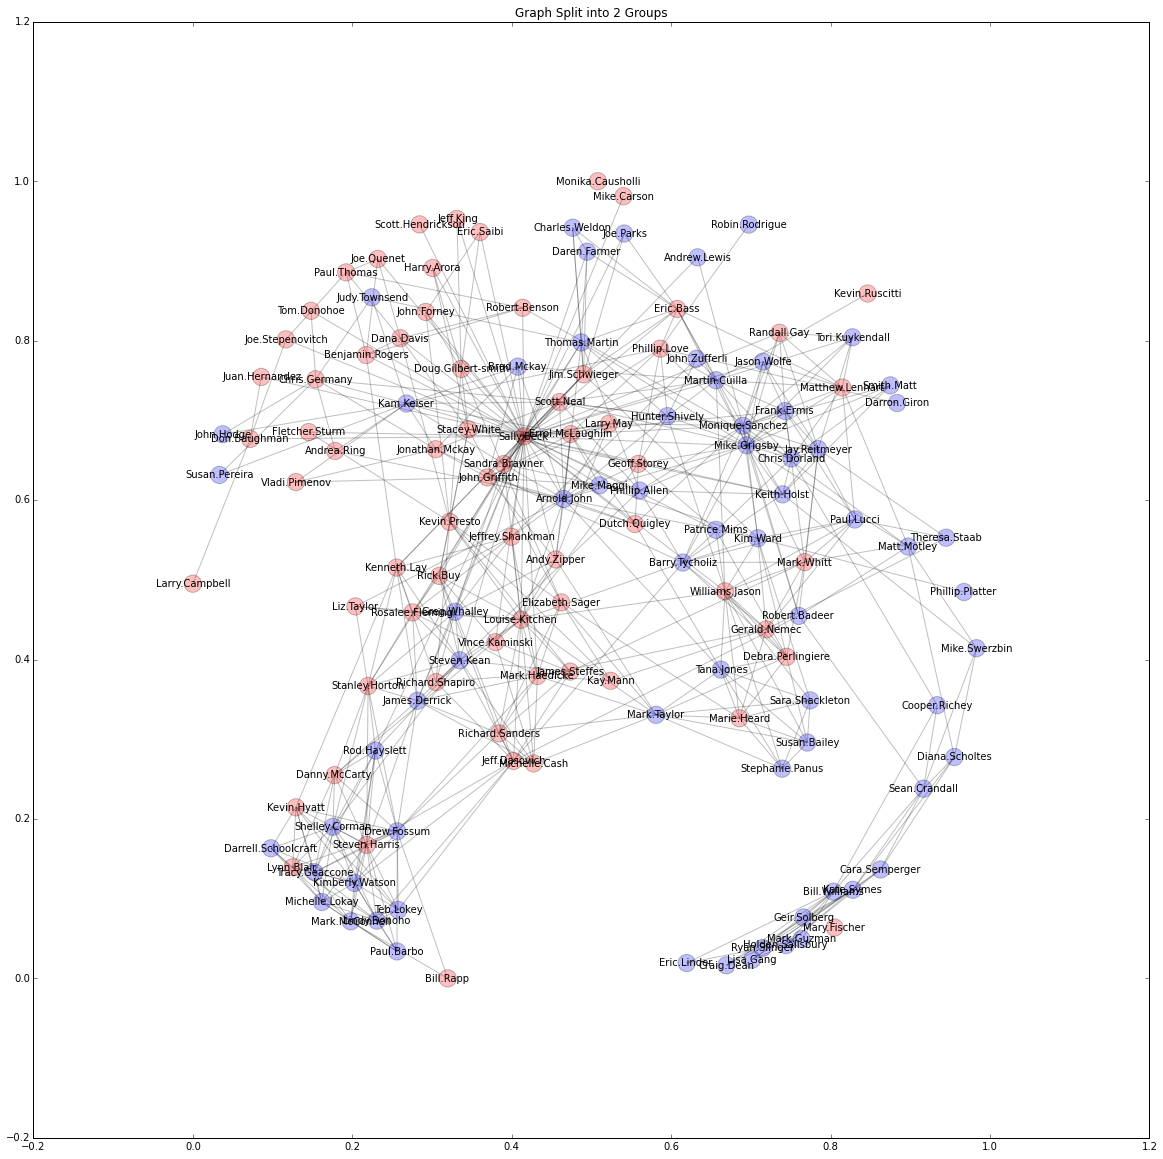
\includegraphics[width=1\textwidth]{figureEnronPartition}
	
	The modularity of this division is 0.16. As previously mentioned a positive number means there is homophily in the network. 
	
	\subsection{Modularity Maximization Using Spectral Techniques} 
	We can also use the idea of modularity to find communities within a network. As discussed earlier modularity is defined as 
	\begin{equation}
		Q = \frac{1}{2m} \sum_{i,j} \left( A_{ij} - \frac{k_i k_j}{2m} \right) \delta (c_i,c_j)
	\end{equation}
	or
	\begin{equation}
		Q = \frac{1}{2m} \sum_{i,j} B_{ij} \delta (c_i,c_j)
	\end{equation}
	\\
	We set up a vector $s$ in the same fashion as we did in the previous section so that $\delta (c_i,c_j)$ = $\frac{1}{2} (s_i s_j + 1)$. Substituting that back into the definition of modularity we get
	\begin{equation}
		Q = \frac{1}{4m} s^T B s
	\end{equation}
	This equation is once again of a similar form as the cut size equation in the previous section. 
	\\
	To solve this optimization problem we once again relax the constraint on $s$ to only take values of +/- 1 and allow $s$ to be any number subject to $|s|$ = $\sqrt{n}$. Differentiating with respect to the elements of $s$ and introducing a Lagrangian we get
	\begin{equation}
		\frac{\partial}{\partial s_i} 
			\left[ 
			\sum_{jk} B_{jk} s_j s_k 
			+ \beta \left( n - \sum_j s_j^2 \right)
			\right] = 0
	\end{equation}
	which ultimately gives
	\begin{equation}
		B s = \beta s
	\end{equation}
	\\
	In other words $s$ is an eigenvector of $B$. Substituting back into the equation for modularity yields
	\begin{equation}
		Q = \frac{n}{4m} \beta
	\end{equation}
	since $s^T s = n$
	\\
	
	In this case we want to maximize modularity so we need to pick $s$ accordingly. If $u_1$ is the eigenvector corresponding to the largest eigenvalue then we need to maximize $s^T u_1$. The best we can do is make each term in $s^T u_1$ positive. So if $u_{1_i}$ is negative we set $s_i$ to be -1 and +1 otherwise. This give us a relatively simple algorithm whereby we only need to look at the sign of each element of the eigenvector corresponding to the largest eigenvalue of the modularity matrix to find partitions in the data. 
	
	This technique can also be applied repeatedly to divide the network into more than two partitions. Applying this technique to the Enron network using data from October 2001 we get
	
	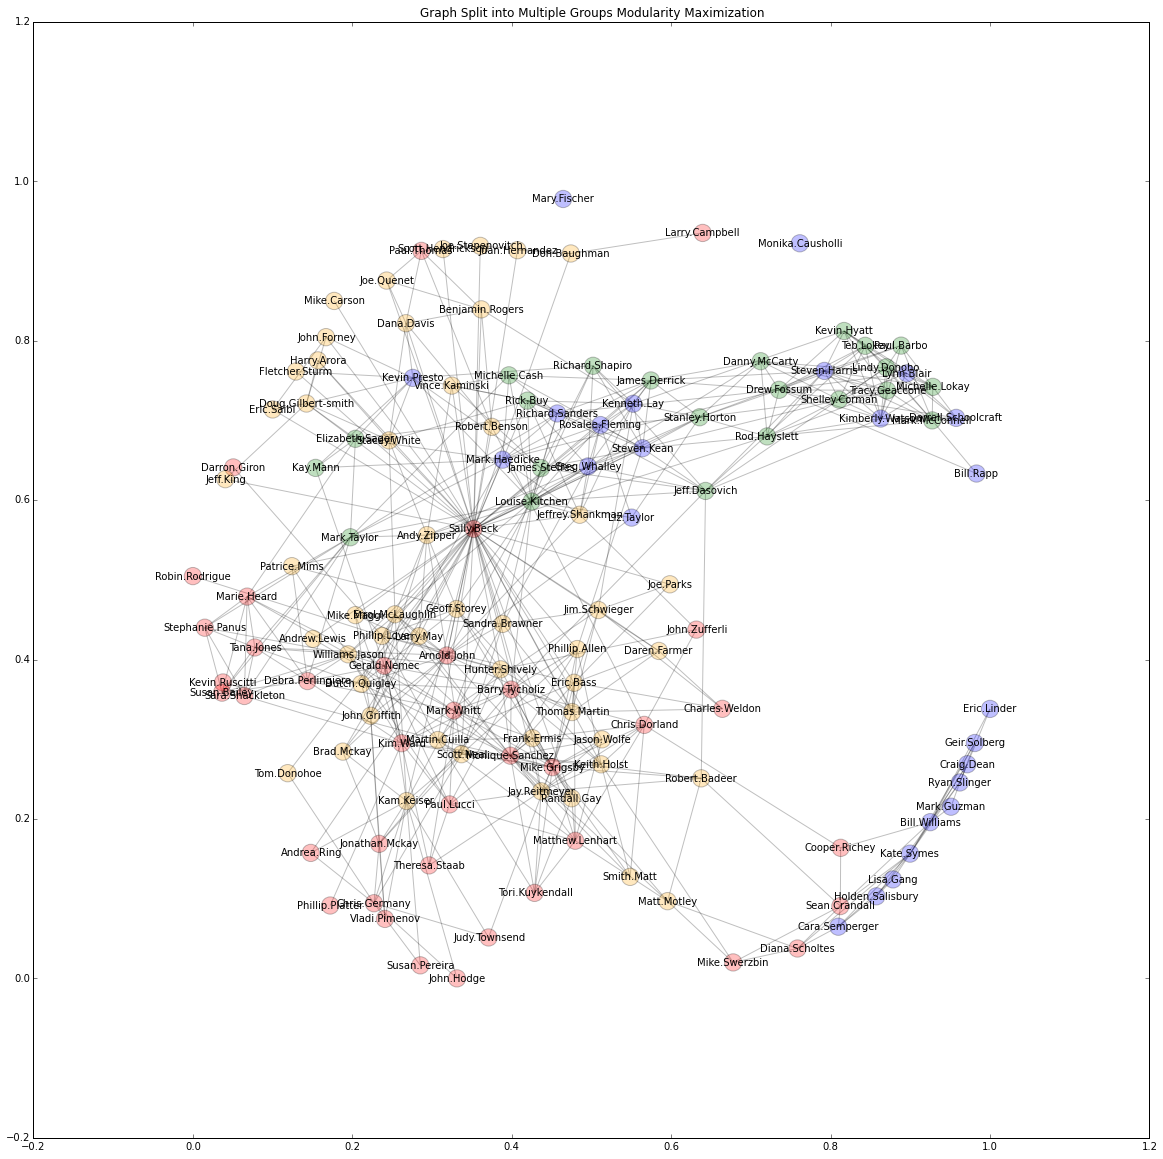
\includegraphics[width=1\textwidth]{figureEnronPartitionMult}



	\subsection{Singular Value Decomposiiton}
		A given $nxn$ adjacency matrix $A$ can be written as
		\begin{equation}
		A = U\Sigma V^T = \sum\limits_{j=1}^n  \sigma_j u_j v_j^T		
		\end{equation}
		where $U$ and $V$ are orthonormal matrices containing the left and right singular vectors of $A$ and $\Sigma$ contains singular values $\sigma_j$ on the diagonal. The summation representation suggests that matrix $A$ can be decomposed as the sum of a weighted combination of matrices. If there exist $\sigma_i$ for $i\in[1,n]$ of significantly larger magnitude than the complement set, we can construct a low rank approximation of matrix $A$ with only these terms in the sum. In the following figure we observe the singular values from the SVD of the directed adjacency matrix defined by the Enron network over the entire 3 year span of the data. Note that we filter the data to include only those sender-receiver relationships in which at least 30 e-mails have been exchanged, and at least 6 e-mails have been sent by each individual.		

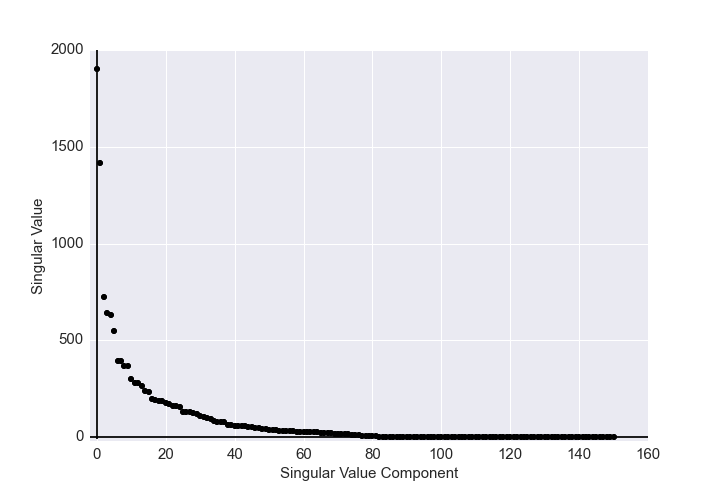
\includegraphics[width=1\textwidth]{SingularValues}

Of particular interest is the dimensionality reduction from $\mathbb{R}^n$ to $\mathbb{R}^2$, as it lends itself to visualization. In this case, we observe two singular values that dominate the rest. We therefore examine the projection of the network to these two dimensions.

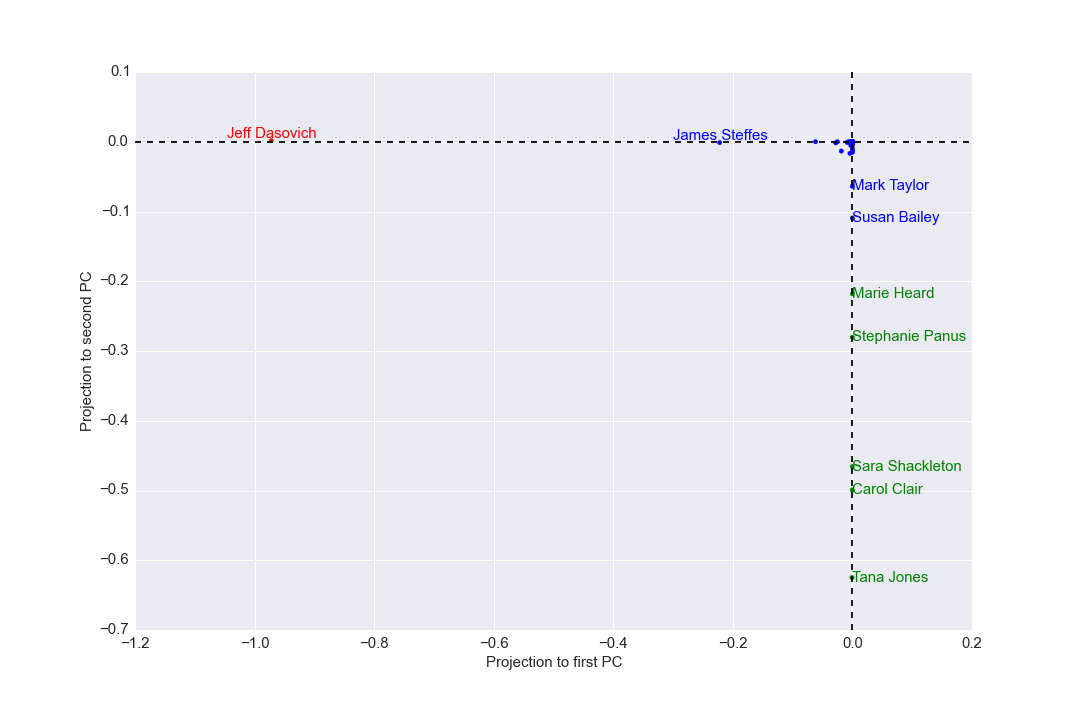
\includegraphics[width=1\textwidth]{ProjectionPC}

Employees are indicated by points on the graph, with the vast majority of points clustered around the origin. Those who stand out under either projection are labeled by name. Initial inspection suggested  clustering, so a K-means algorithm with K= 3 was used. The three groups are color coded. Interestingly, Jeff Dasovich and James Steffes were two of the only members in the network whose work revolved around government relations. Furthermore, Tana Jones, Carol Clair, Stephanie Panus, Marie Heard, Susan Bailey, and Mark Taylor comprised a majority of the legal team present in the network during these three years. Therefore, we have identified distinct groups of employees using unlabeled data whose titles suggest particular importance in managing Enron's external relations.


\section{Evolution Across Time} As with any social network, the dynamics at Enron were constantly changing. The time course of e-mail exchanges provides insight into these dynamics. We calculated several informative metrics on the network for each month from May 1999 to June 2002. 

\subsection{Metrics}

\begin{itemize}

\item Number of nodes and edges
\begin{itemize}
\item These represent the number of employees and the number of e-mail exchanges between employees respectively.
\end{itemize}


\item Size of giant component
\begin{itemize}
\item Many networks exhibit a core-periphery structure whereby a large connected cluster of nodes exists centrally and isolated sub-components exist around it. The main connected component is referred to as the giant component. One metric of size is the diameter of a graph. This is defined as the maximum eccentricity of the graph. The eccentricity of a node is the maximum shortest path between that node and every other node in the network. Therefore, the diameter of the giant component refers to the maximum shortest path between any two nodes in the connected graph.
\end{itemize}


\item Percent of nodes in giant component
	\begin{itemize}
		\item This is a measure of the extent to which core-periphery structure is present.
	\end{itemize}

\item Average shortest path length within the giant component
	\begin{equation}
		a = \sum\limits_{s,t\in V}  \frac{d(s,t)}{n(n-1)}		
	\end{equation}
where $d(s,t)$ is the shortest path from $s$ to $t$, and $n$ is the number of nodes in the graph  \cite{networkx}.

\item Average clustering coefficient
	\begin{itemize}
		\item The average is taken across the clustering coefficient calculated on each node as,
		\begin{equation}
		c_u = \frac{2T(u)}{deg(u)(deg(u)-1)}		
		\end{equation}
		
		where $T(u)$ is the number of triangles through node $u$ and $deg(u)$ is the degree of $u$  \cite{networkx}.
		A common feature of social networks is dense local clustering with only a few edges between clusters. This has been characterized as the "small world phenomenon," because most people are in contact with only a small subset of the network, but they are acquaintances with a few individuals who are connected to other dense clusters. Therefore, the degree of separation across the network is not as high as might be expected.		
		
	\end{itemize}
\item Magnitude of power in the degree distribution \cite{newman}

\item Of the approximately one billion web pages on the World Wide Web, most are isolated, and many are obsolete. Only a few are truly central to the ongoings of the Internet. If we characterize this as a network with web pages as nodes and links as edges, we can capture this intuition through a determination of the the distribution of degrees across nodes. It has been shown that a power law relationship exists between the number of links and the number of webpages. More accurately, the Web encompasses a directed graph and the power law nature is found in both the in-degree (number of links to other websites) and out-degree distribution (number of links to the website). The joint distribution for the Enron e-mail network is shown here:

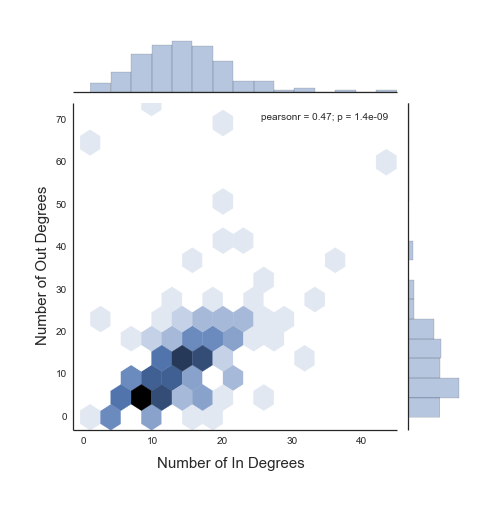
\includegraphics[width=1\textwidth]{JointDegreeDistribution}

Networks that exhibit power law behavior are called "scale-free" networks, and have been studied extensively for their special properties. The characteristic high degree nodes are called "hubs," and, in the context of the Enron network these are the individuals with the most connections to others. Note that there is a clear distention between this feature and the centrality measures mentioned previously. The power law nature of the Enron graph is demonstrated for one month in time:
For a power law defined as:

	\begin{equation}
		p_k = ck^{-\alpha}		
	\end{equation}


the logarithm will be linear:

	\begin{equation}
		log(p_k) = log(c)-\alpha log(k)		
	\end{equation}
	
with the slope equal to the power.
The log of the degree distribution across the 3 year period is shown here, along with the best-fit line. 

\includegraphics[width=1\textwidth]{LinearDegree}


\end{itemize}



\subsection{Network Dynamics and Associated Timeline of Events}

\includegraphics[width=1\textwidth]{Timeseries}


%\newpage
The following timeline of events was adapted from a New York Times article \cite{nyttimeline}:
\renewcommand{\theenumi}{\Alph{enumi}}
\begin{enumerate}
\item August 2000 - Enron shares reach high of \$90.\\
\item February 2001 Jeff Skilling succeeds Kenneth Lay as CEO, stock hits 52-week high.\\

\item August  2001
	\begin{itemize}
		\item Aug 14: Skilling resigns (6 months after becoming CEO); Lay named CEO again.
		\item Aug 22: Finance executive Sherron Watkins meets privately with Lay to discuss concerns of murky finance and accounting that could ruin the company.
\end{itemize} 

\item October 2001
\begin{itemize}
	\item Oct. 16: Enron announces \$638 million in third-quarter losses and a \$1.2 billion reduction in shareholder equity as well as unwinding of financial entities designed to keep hundreds of millions of dollars in debt off the books.\\
	\item Oct. 19: Securities and Exchange Commission launches inquiry into Enron finances.\\
\end{itemize}

October 2001 is the point when imminent failure became a likelihood, and it is captured by the metrics shown above. The number of nodes and edges are maximized here, which is indicative of increased communication amongst the network. Every employee is in the core structure of the network, and no one is isolated. The average path length dips, which is expected because of increased connection between employees. Most markedly, the degree distribution is not nearly as subject to an exponential decay, which means there was an increase in the number of individuals who were exchanging many e-mails with others. 

\item November 2001
\begin{itemize}
	\item Nov. 8: Enron files documents with SEC revising its financial statements for previous five years to account for \$586 million in losses.
	\item Nov. 9: Dynegy Inc. announces an agreement to buy Enron for more than \$8 billion in stock.
	\item Nov. 19: Enron restates its third-quarter earnings and discloses a \$690 million debt is due Nov. 27.
	\item Nov. 28: Enron stock plunges below \$1 as Dynegy Inc. aborts its plan to buy its former rival.
\end{itemize}

\item December 2, 2001 - Enron goes bankrupt, thousands of workers laid off.

\item January 2002
\begin{itemize}
	\item Jan. 9: Justice Department confirms it has begun a criminal investigation of Enron.
	\item Jan. 23: Lay resigns as chairman and CEO.
\end{itemize}

\end{enumerate}



\section{Conclusions}
	We were able to identify key actors at Enron simply by analyzing the data rather than looking at complicated organizational charts. The centrality measures we considered were able to extract important individuals even when they did not exchange many e-mails with other employees. While some people (like CEO Ken Lay) are known to have had a major impact on the company, network analysis lets us identify those among the subordinate majority who play an influential role.
	
	Within the graph theoretic construct, a natural analysis of social networks is the detection of communities. Most real world networks exhibit some form of clustering, and identifying this underlying structure (and identifying why it exists) can be valuable in a range of applications. Here, we looked at three methods of community detection that suggested possible delineations within the network. Using SVD, we identified two groups consisting of government relations experts and legal counselors that emerged as significant factors. In practice, interpreting these groups of people might require specific knowledge about the company but it can help unearth connections between people that might have been missed.
	
	The Enron e-mail data set captures the company in its heyday and its very rapid, very public demise. A longitudinal analysis of such data allows us to explore the organizational structure of a large corporation, the major events that lead to paradigm shifts, and the restructuring afterwards. In this analysis, we noted a slight trend toward increased connectivity and density of the network followed by a marked shift in network metrics when news of the potential fraud was made public. Such analysis can be useful in event detection and prediction thereof.
	
	Interpretation of the data beyond what we were able to provide here may be achieved with additional information about, for example, where employees were geographically located. Additionally, we implemented multiple methodologies on a limited set of permutations of the available data, but some subsets of data may be more telling of the company's ongoings. Between an expansive and growing array of intriguing network analysis methodologies, and this unique, fascinating data set, there are many exciting opportunities for continued investigation. 


\begin{thebibliography}{9}

\bibitem{ferc}
http://www.ferc.gov/industries/electric/indus-act/wec/enron/info-release.asp

\bibitem{Diesner}
http://research.cs.queensu.ca/~skill/proceedings/diesner.pdf

\bibitem{Chapanond}
http://research.cs.queensu.ca/~skill/proceedings/yener.pdf

\bibitem{Priebe}
http://research.cs.queensu.ca/~skill/proceedings/priebe.pdf

\bibitem{npr}
http://www.npr.org/news/specials/enron/

\bibitem{shetty}
Shetty, J., Adibi, J. (n.d.). The Enron Dataset
Database Schema and Brief Statistical Report

\bibitem{pfeiffer}
https://www.cs.purdue.edu/homes/jpfeiff/enron.html
data retrieved on Nov 11 2014

\bibitem{nyt}
http://www.nytimes.com/2006/01/18/business/worldbusiness/18iht-web.0117enron.time.html

\bibitem{park}
http://cis.jhu.edu/~parky/Enron/employees

\bibitem{newman}
Networks: An Introduction by M.E.J Newman

\bibitem{networkx}
https://networkx.github.io/documentation/latest/index.html

\bibitem{nyttimeline}
http://www.nytimes.com/2006/01/18/business/worldbusiness/18iht-web.0117enron.time.html?pagewanted=all



\end{thebibliography}


\end{document}
